% vim: spelllang=en
\section{Conduction}%
\label{sec:conduction}
\begin{wrapfigure}{r}{0.6\textwidth}
		\centering
		\includegraphics[width=1.0\linewidth]{./build/emissionconstruction.pdf}
		\caption{Sketch of the setup to check if the laser produces induced or
		spontaneous emission. \cite{anleitung}}
		\label{fig:aufbau}
\end{wrapfigure}
Goal of the experiment is to adjust a laser, so that it can be used for further
observation.
% For further observation with a laser, you have to adjust it first.
First task is to calibrate the current of the laser diode to achieve population inversion.
For making the laser light visible the laser is pointed to a IR-card,
which is filmed by a charge coupled device (ccd sensor).
To achieve the minimal current to lase by induced emission, alternately the head
knob and side knob positions are optimized.
Every time when stimulated emission is produced, the laser current is reduced a
little bit.
The last visible induced emission is an estimation of the minimal laser current.
Characteristic for induced emission is that the light cone is
much brighter and more homogeneous than from spontaneous emission.
One example for induced~(\ref{fig:induce}) and spontaneous~(\ref{fig:spontanious}) light cone is
shown in figure~\ref{fig:emission}.
\begin{figure}[ht]
		\centering
		\begin{subfigure}[b]{0.45\textwidth}
				\begin{center}
						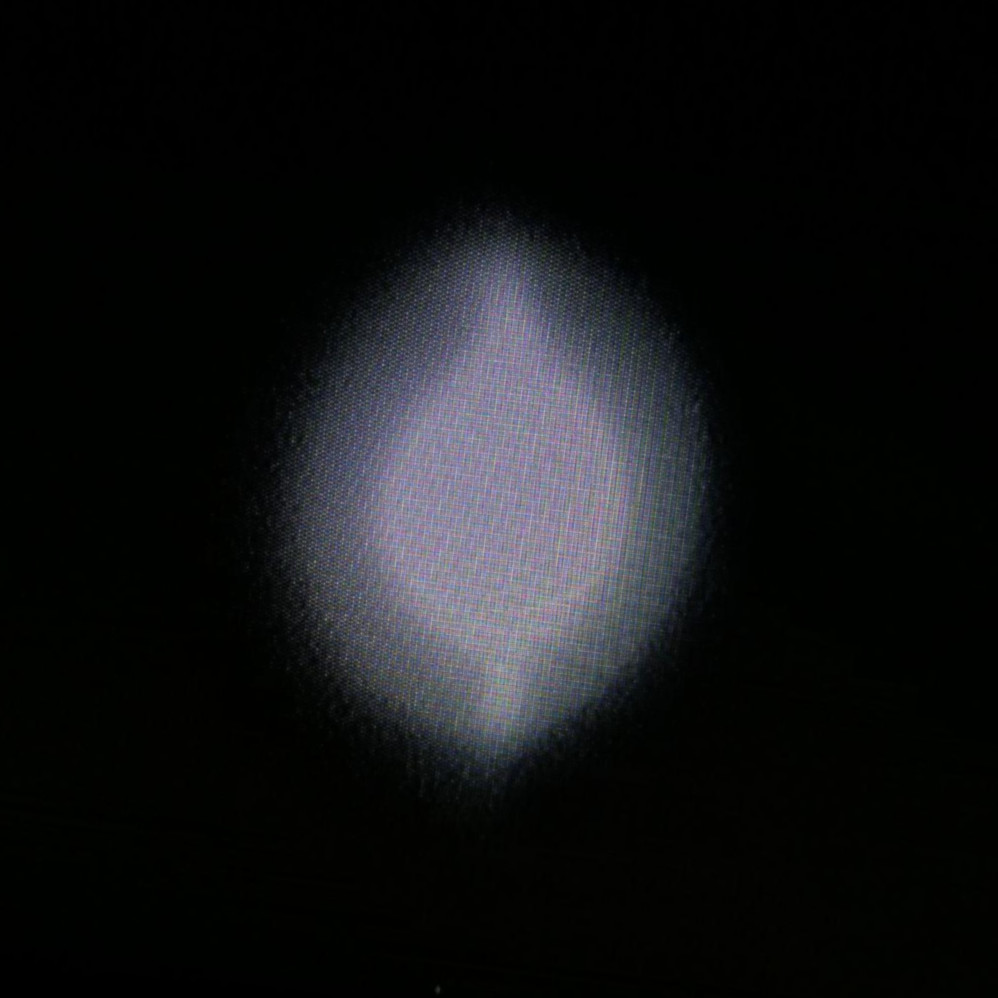
\includegraphics[width=0.7\linewidth]{./content/pictures/below_threshold.jpg}
						\caption{Spontaneous emission}
				\label{fig:spontanious}
				\end{center}
		\end{subfigure}
		\begin{subfigure}[b]{0.45\textwidth}
				\begin{center}
						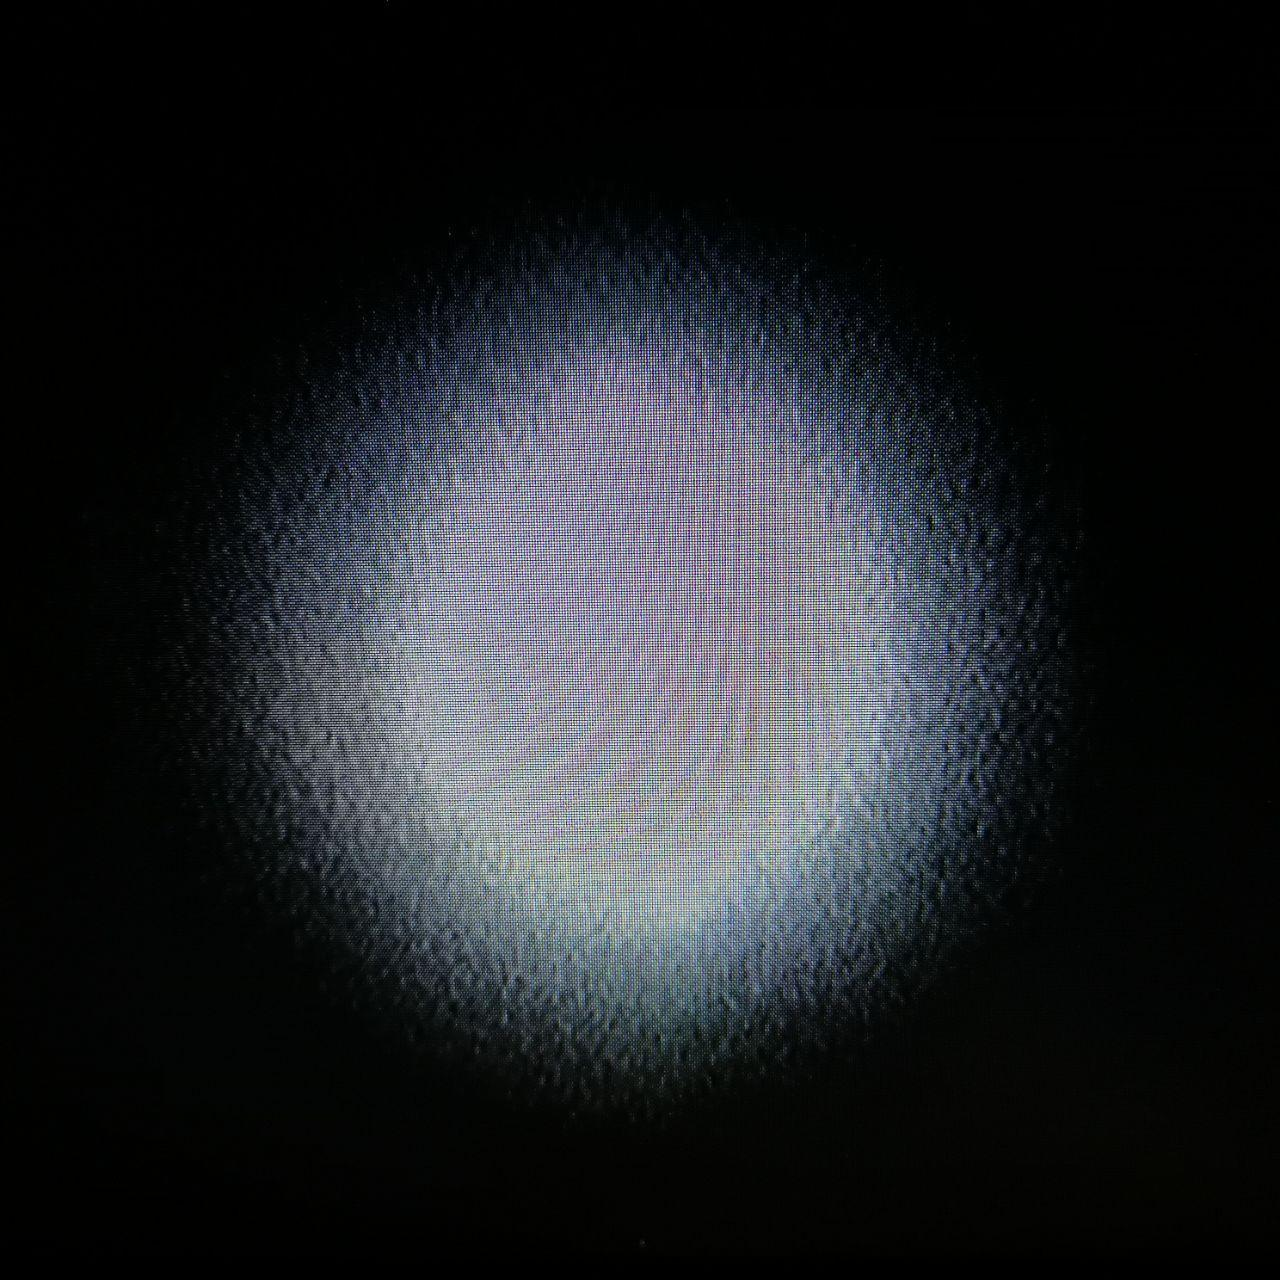
\includegraphics[width=0.7\linewidth]{./content/pictures/above_threshold.jpg}
						\caption{Induced emission}
						\label{fig:induce}
				\end{center}
		\end{subfigure}
		\caption{Light emission of a diode laser visible on a fluorescence
		paper observed by a ccd camera.}
		\label{fig:emission}
\end{figure}
The measured current for the minimal threshold is
\begin{align}
  I_0 &= \SI{30}{\milli\ampere}.
\end{align}
By moving both knobs over full range, no more flashes can be generated.

\subsection{Fluorescence rubidium}%
\label{sub:anregen_rubidium}

To stimulate the rubidium gas the beam has to pass the chamber without contact
to the border of the chamber.
Figure~\ref{fig:hole_emission} shows how the measuring instruments have to be
arranged to measure the light intensity.
\begin{figure}[ht]
		\centering
		\includegraphics[width=0.8\linewidth]{build/rubidiumemission.pdf}
		\caption{Sketch of a setup to measure the spectrum of Rubidium and
		aligning the laser on right frequency.\cite{anleitung}}%
		\label{fig:hole_emission}
\end{figure}
A photo diode is placed behind the Rb-cell to measure the laser light which
passes the cell.
The voltage of the photo diode is increased and shown on an oscilloscope.
The grating can be rotated with the side knob to change the length of the
cavity to attain the right frequency for stimulating the gas.
A grating is put into the beam to reduce the contrast so that the beam angle
can be seen with the help of a ccd camera.
If in the camera a small beam is visible, the desired frequency is found.
% Da der Resonator mehrere Moden besitzt werden die Eigenfrequenzen des
% Resonators gesucht bei dem das Gas stimuliert wird und die mittlere der
% Frequenen gewählt, da diese die größte Verstärkung besitzt.
Different eigenfrequencies can be generated in the spectrum of the
cavity to produce stimulated emission.
The middle one is chosen because it has the strongest gain.
\begin{figure}[ht]
		\centering
		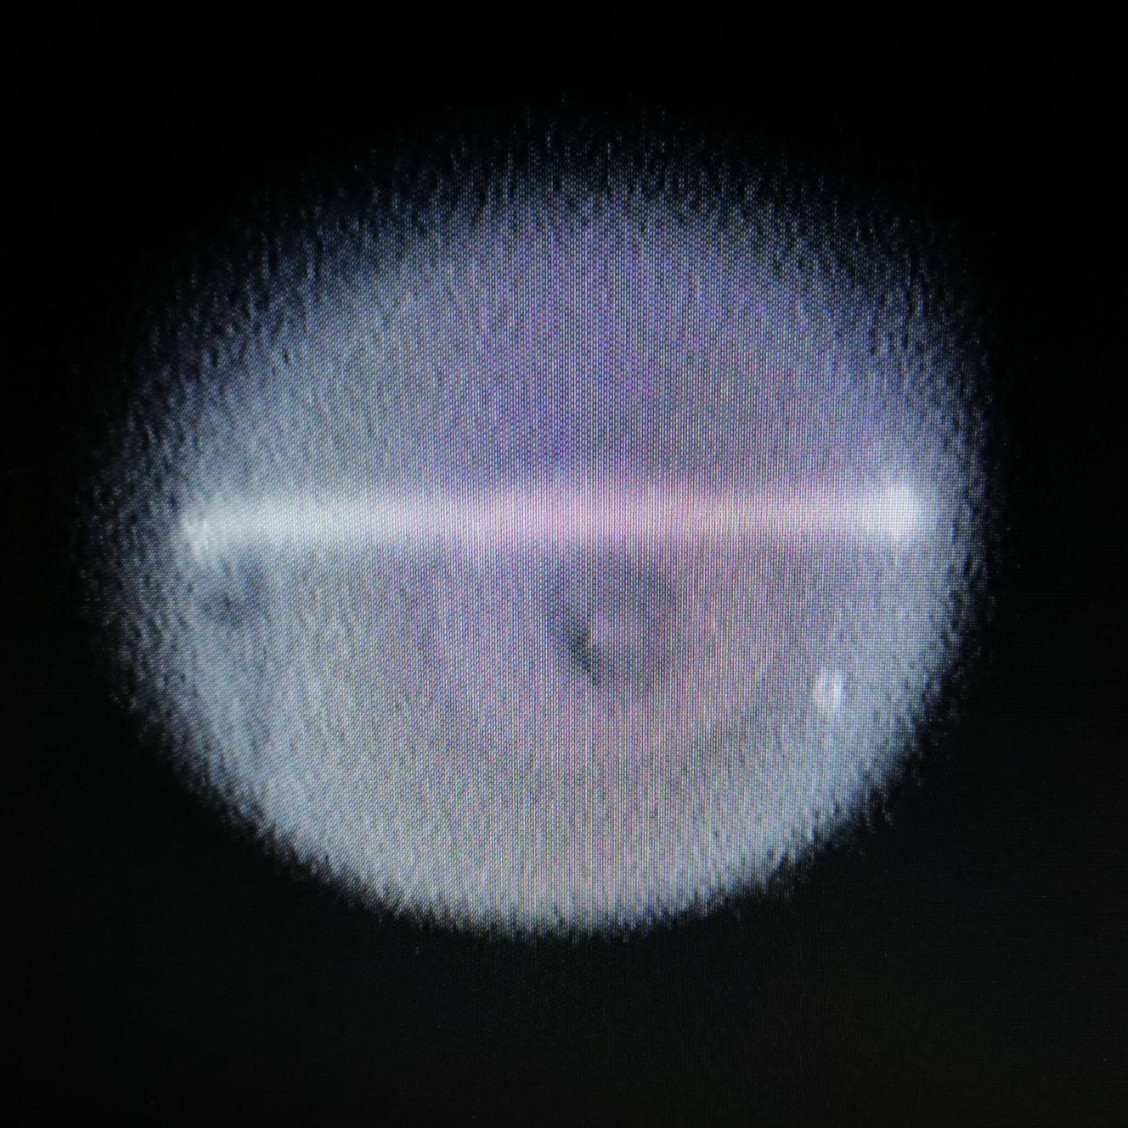
\includegraphics[width=0.4\linewidth]{./content/pictures/fluorescence.jpg}
		\caption{Fluorescence of rubidium filmed by ccd camera with
				\SI{69.9}{\milli\ampere} laser current.}%
		\label{fig:ionized}
\end{figure}
An example for fluorescing rubidium is shown in figure~\ref{fig:ionized}.
After the rubidium is fluoresced, the goal is to measure the absorption spectrum.

\subsection{Absorption spectrum}%
\label{sub:absorbtion_spectrum}
% Um die Resonanzstellen des Gases zu treffen muess der Resonator durchgestimmt
% werden.
To find the resonance of the gas, the cavity modes has to be tuned.
To achieve a variation in frequency a piezo element is used.
The piezo element is at the diffraction grating to variate the length of the
external cavity.
Variation of cavity length causes shifts in laser frequency.
The piezo element is powered by a ramp generator which causes linear shifts in
cavity length in a defined time period.
When photon current is measured by a sensor the dependency between piezo voltage and
transmission can be plotted.
\begin{figure}[ht]
		\centering
		\begin{subfigure}[b]{0.49\textwidth}
				\begin{center}
				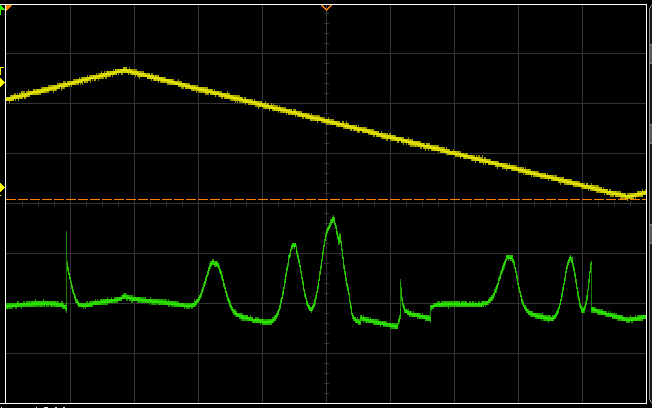
\includegraphics[width=1.0\linewidth]{./content/pictures/scope_136.png}
						\caption{Mode hopping}%
				\label{fig:piezotest}
				\end{center}
		\end{subfigure}
		\begin{subfigure}[b]{0.49\textwidth}
				\begin{center}
						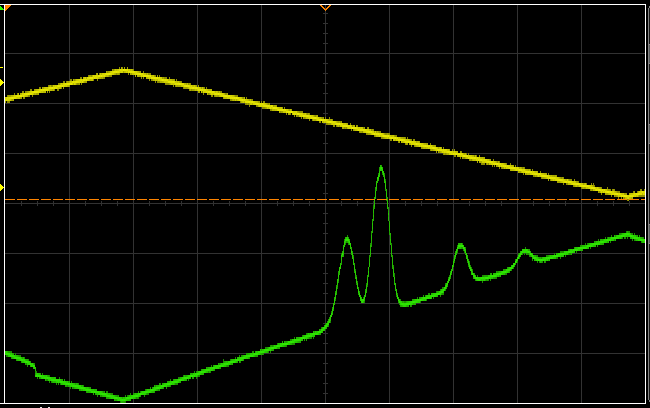
\includegraphics[width=1.0\linewidth]{./content/pictures/scope_138.png}
						\caption{Triangle background}%
						\label{fig:rectangular}
				\end{center}
		\end{subfigure}
		\caption{Absorption spectrum with undesired side effects.}%
		\label{fig:}
\end{figure}
In figure~\ref{fig:piezotest} the yellow line shows the voltage at the piezo
element which causes frequency shifts of the emitted light proportional to
applied voltage.
% Die grüne linie ist der gemessene Photonenfluss. Dieser ist proportinal zum
% Absorptionsspektrum eines mit photonen beschossenen Objektes.
The green line represents the measured photon stream, where peaks are caused by
absorption of rubidium.
Hops in the photon stream are horizontal modes caused by the piezo element.
They are of no further interest.
Mode hopping can be reduced by modulation with the piezo voltage as shown in
figure~\ref{fig:rectangular}.
The characteristic absorption spectrum of rubidium is visible with the
absorption lines.
In general the green line should be mirrored on the x-axis because resonance
reduces the intensity on the photon stream.
To achieve a flat absorption spectrum which is not dependent on the piezo voltage some
modifications are necessary.

\subsection{Modulated spectrum}%
\label{sub:modulated_spectrum}

The beam will be divided into two parts
for modulation of the initial laser beam and that which passes the medium.
A semipermeable mirror will be set in the beam path in front of the medium.
Light which is reflected in front of the medium will be measured by a second photomultiplier.
Now beam modulation with a part which not passes and a part which passes the
medium can be done.
The absorption spectrum without piezo movement effect is shown in figure~\ref{fig:modulation}.
\begin{figure}[ht]
		\centering
		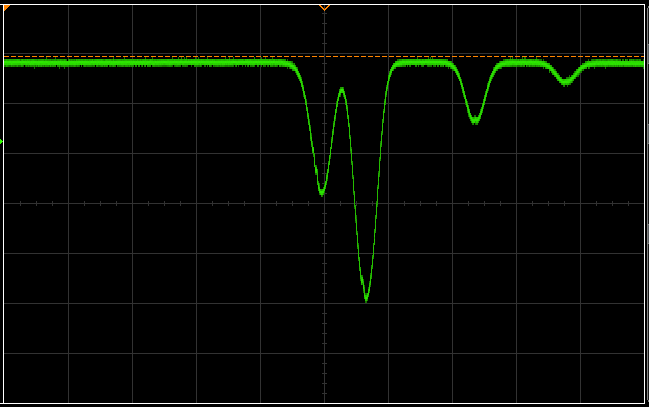
\includegraphics[width=0.8\linewidth]{./content/pictures/scope_140.png}
		\caption{Absorption spectrum of rubidium.}%
		\label{fig:modulation}
\end{figure}
There are the different energy levels (85\sfrac{a}{b}, 87\sfrac{a}{b}) visible.
Gaps in the spectrum correspond to the difference of two energy levels.
Now the laser is aligned and ready for further experiments.
